In the third experiment, human subjects are involved in a grasping
task, which our system must identify; in particular, we are interested
in classifying the grasping posture independently of the subject and
the object being grasped.
%, thus focusing on the \emph{affordances} \cite{gibson} associated with objects.
Eight subjects were involved in
the experiment, $5$ men and $3$ women, all able-bodied, aged between
$23$ and $36$. They were given no prior knowledge on the aim and scope
of the experiment. Each subject would sit comfortably in front of a
workspace large about one squared meter and wear a $22$-sensors
Immersion CyberGlove \cite{cyberglove} on the right hand, and a Force
Resistor Sensor (FSR) on the thumb. Figure \ref{fig:devices} (upper
row) shows the devices, as worn by a subject.

\begin{figure*}[!ht]
  \begin{center}
    \begin{tabular}{c}
      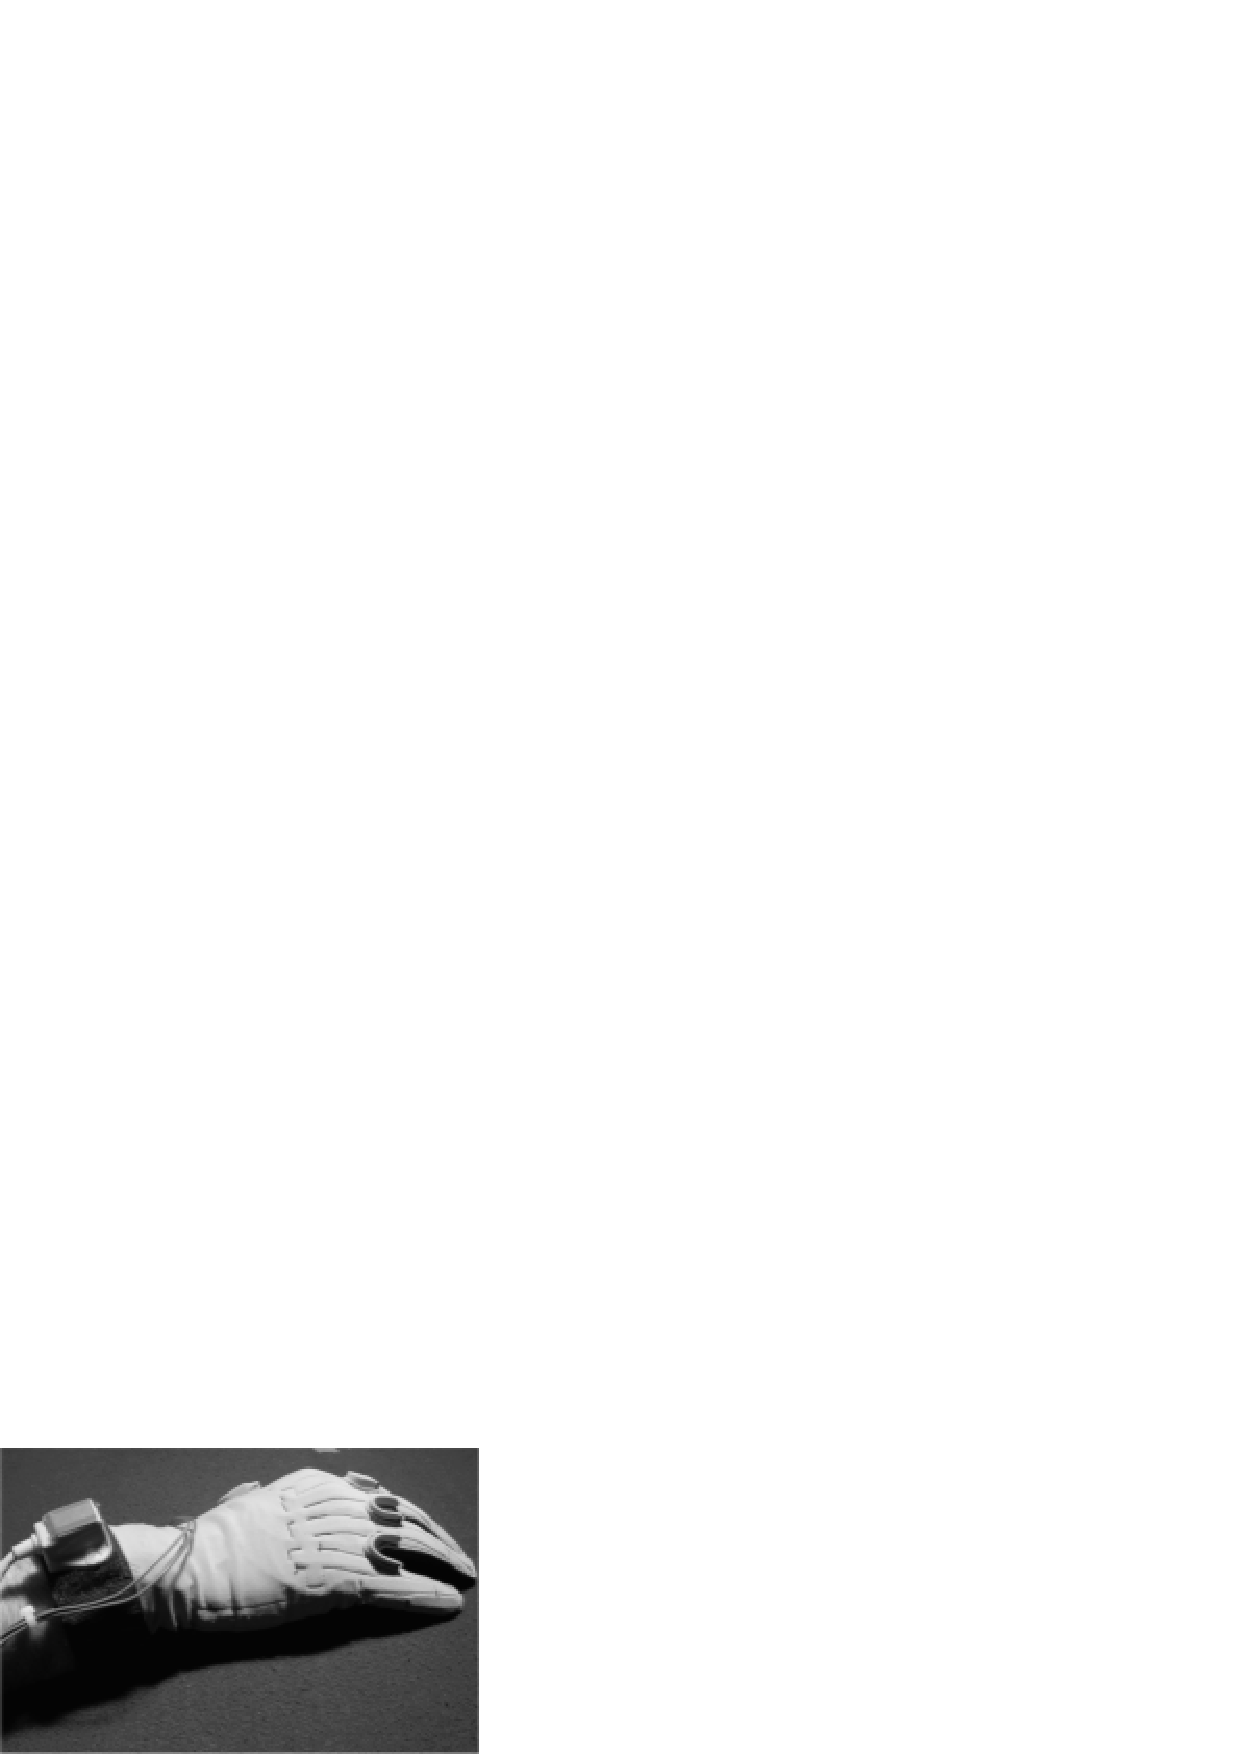
\includegraphics[height=0.08\textheight]{figs/grasping/devices1.jpg}
      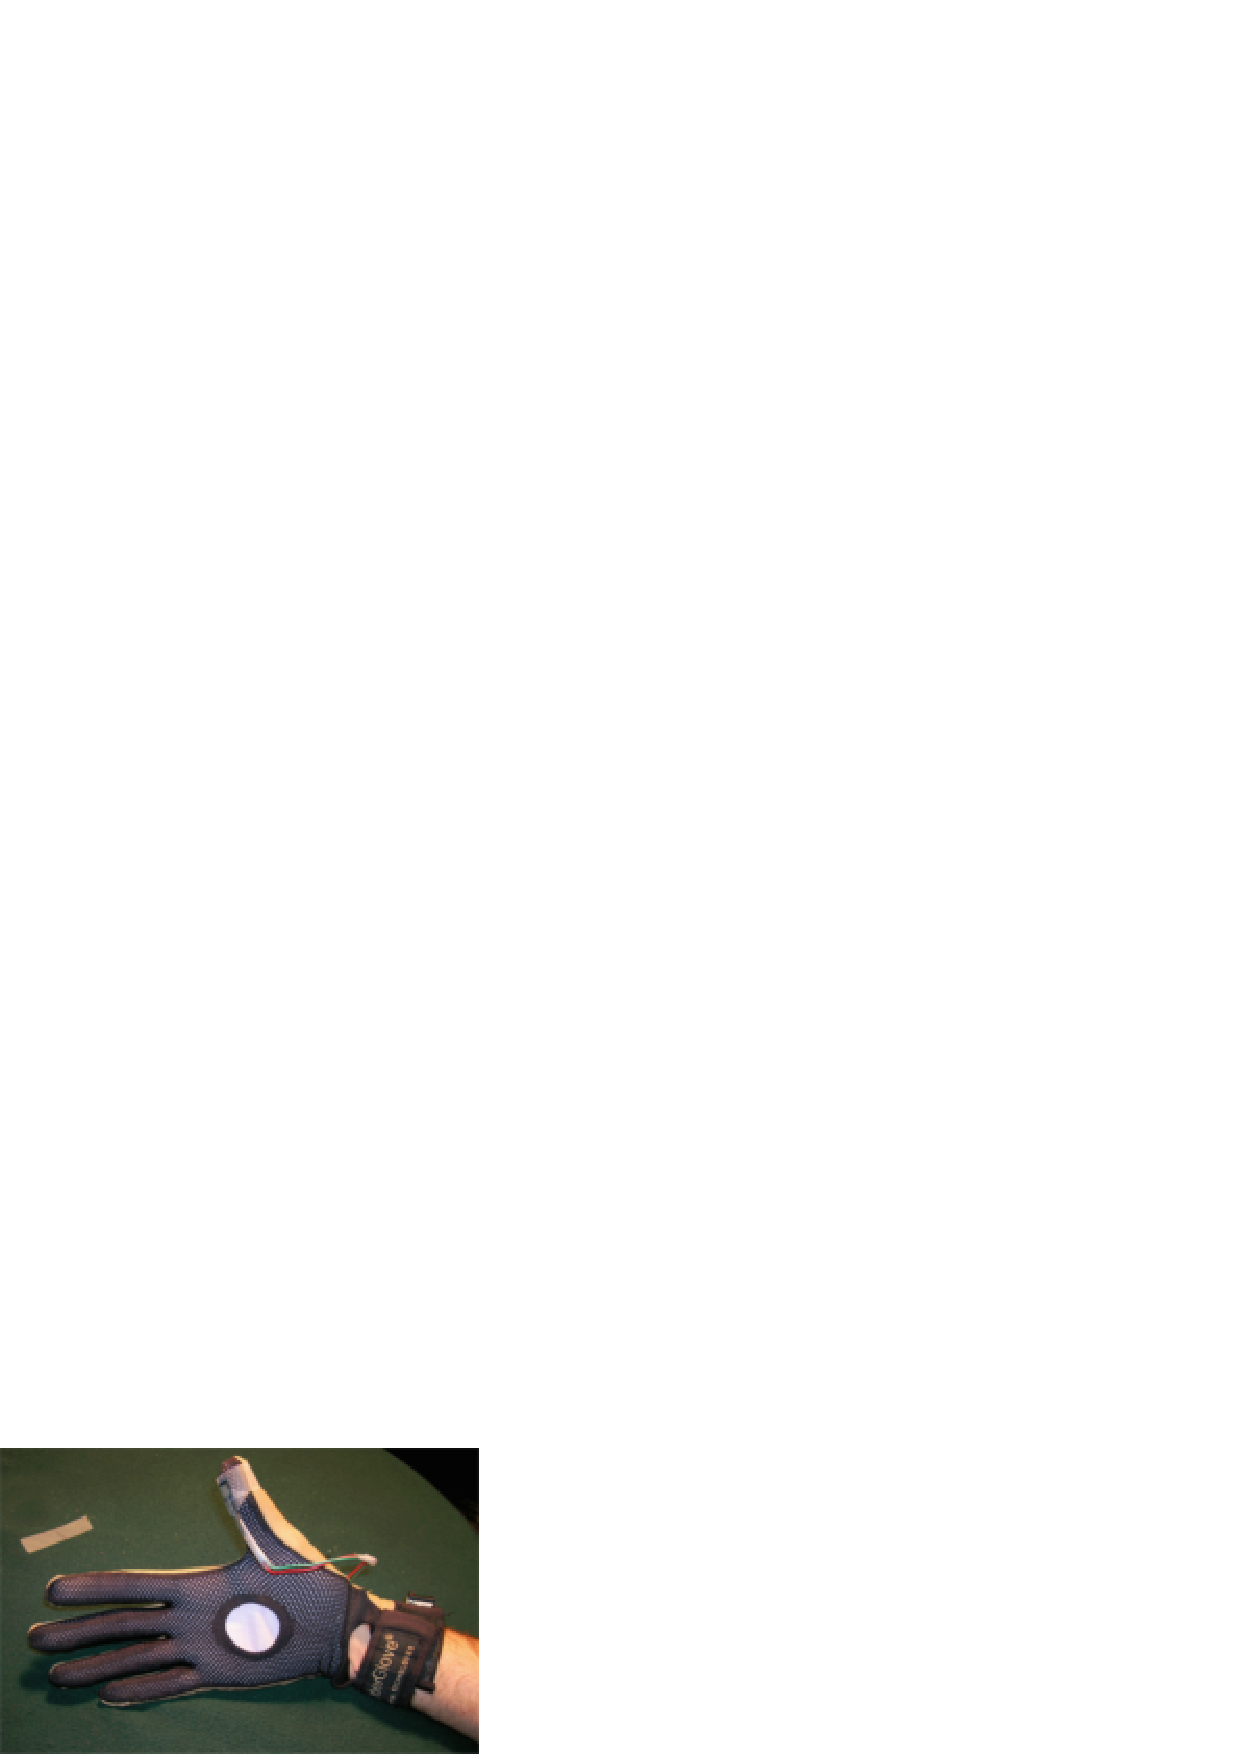
\includegraphics[height=0.08\textheight]{figs/grasping/devices2.jpg}
      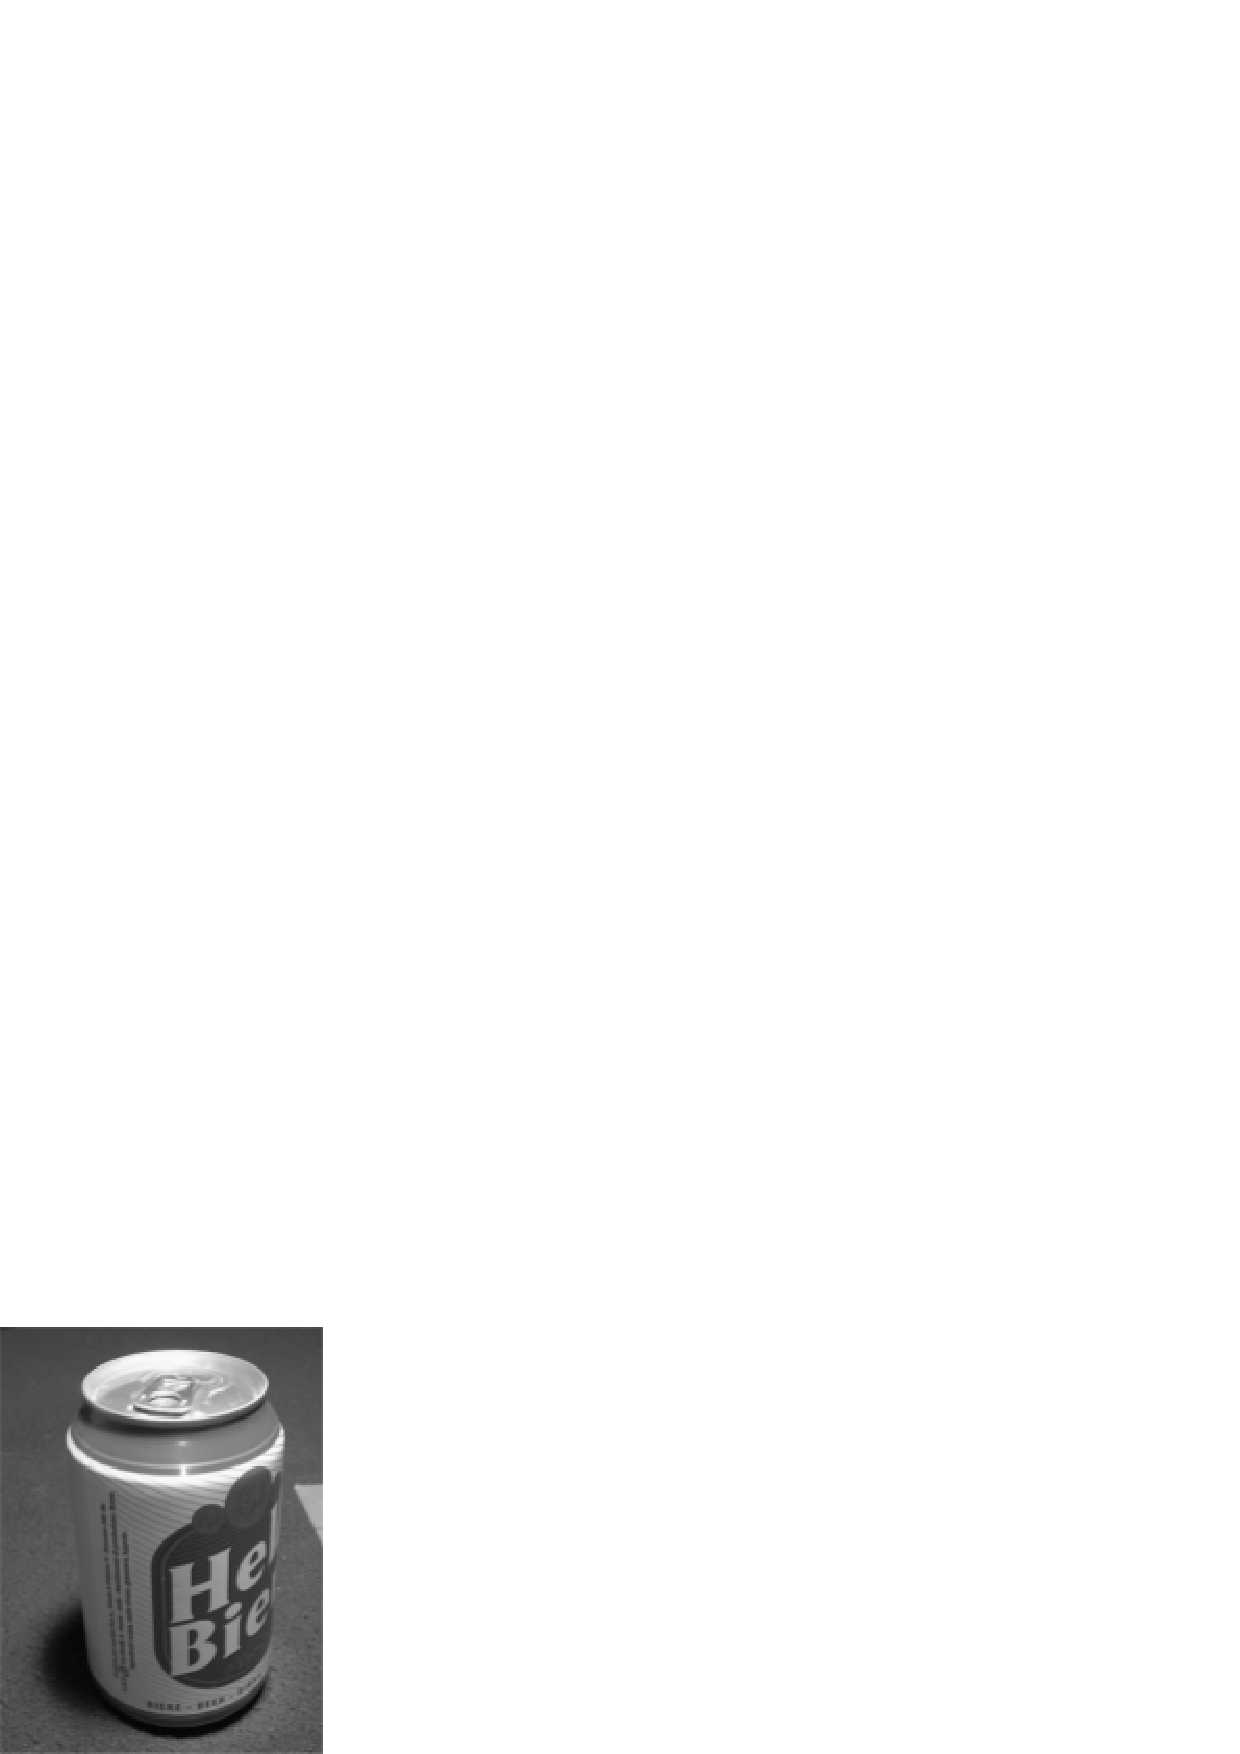
\includegraphics[height=0.08\textheight]{figs/grasping/beer.jpg}
      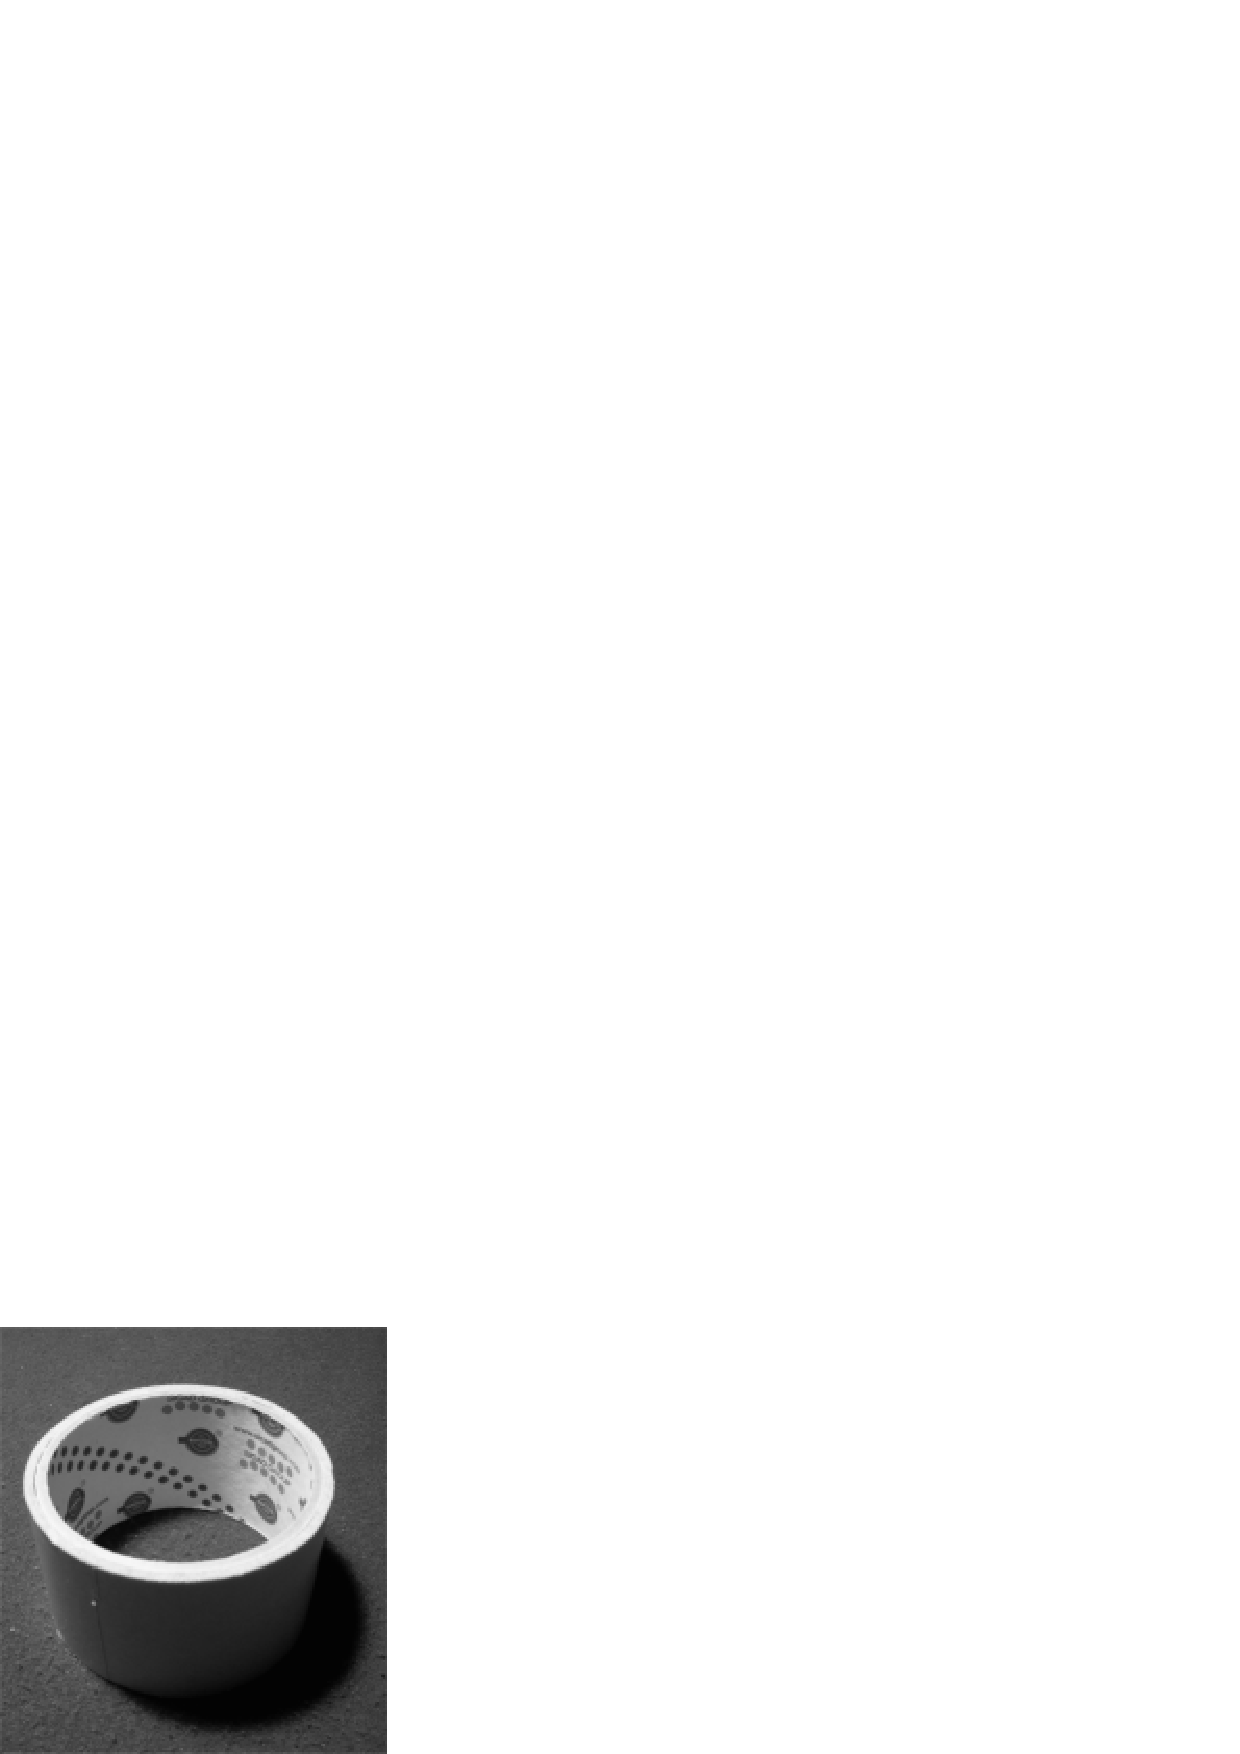
\includegraphics[height=0.08\textheight]{figs/grasping/scotch.jpg}
      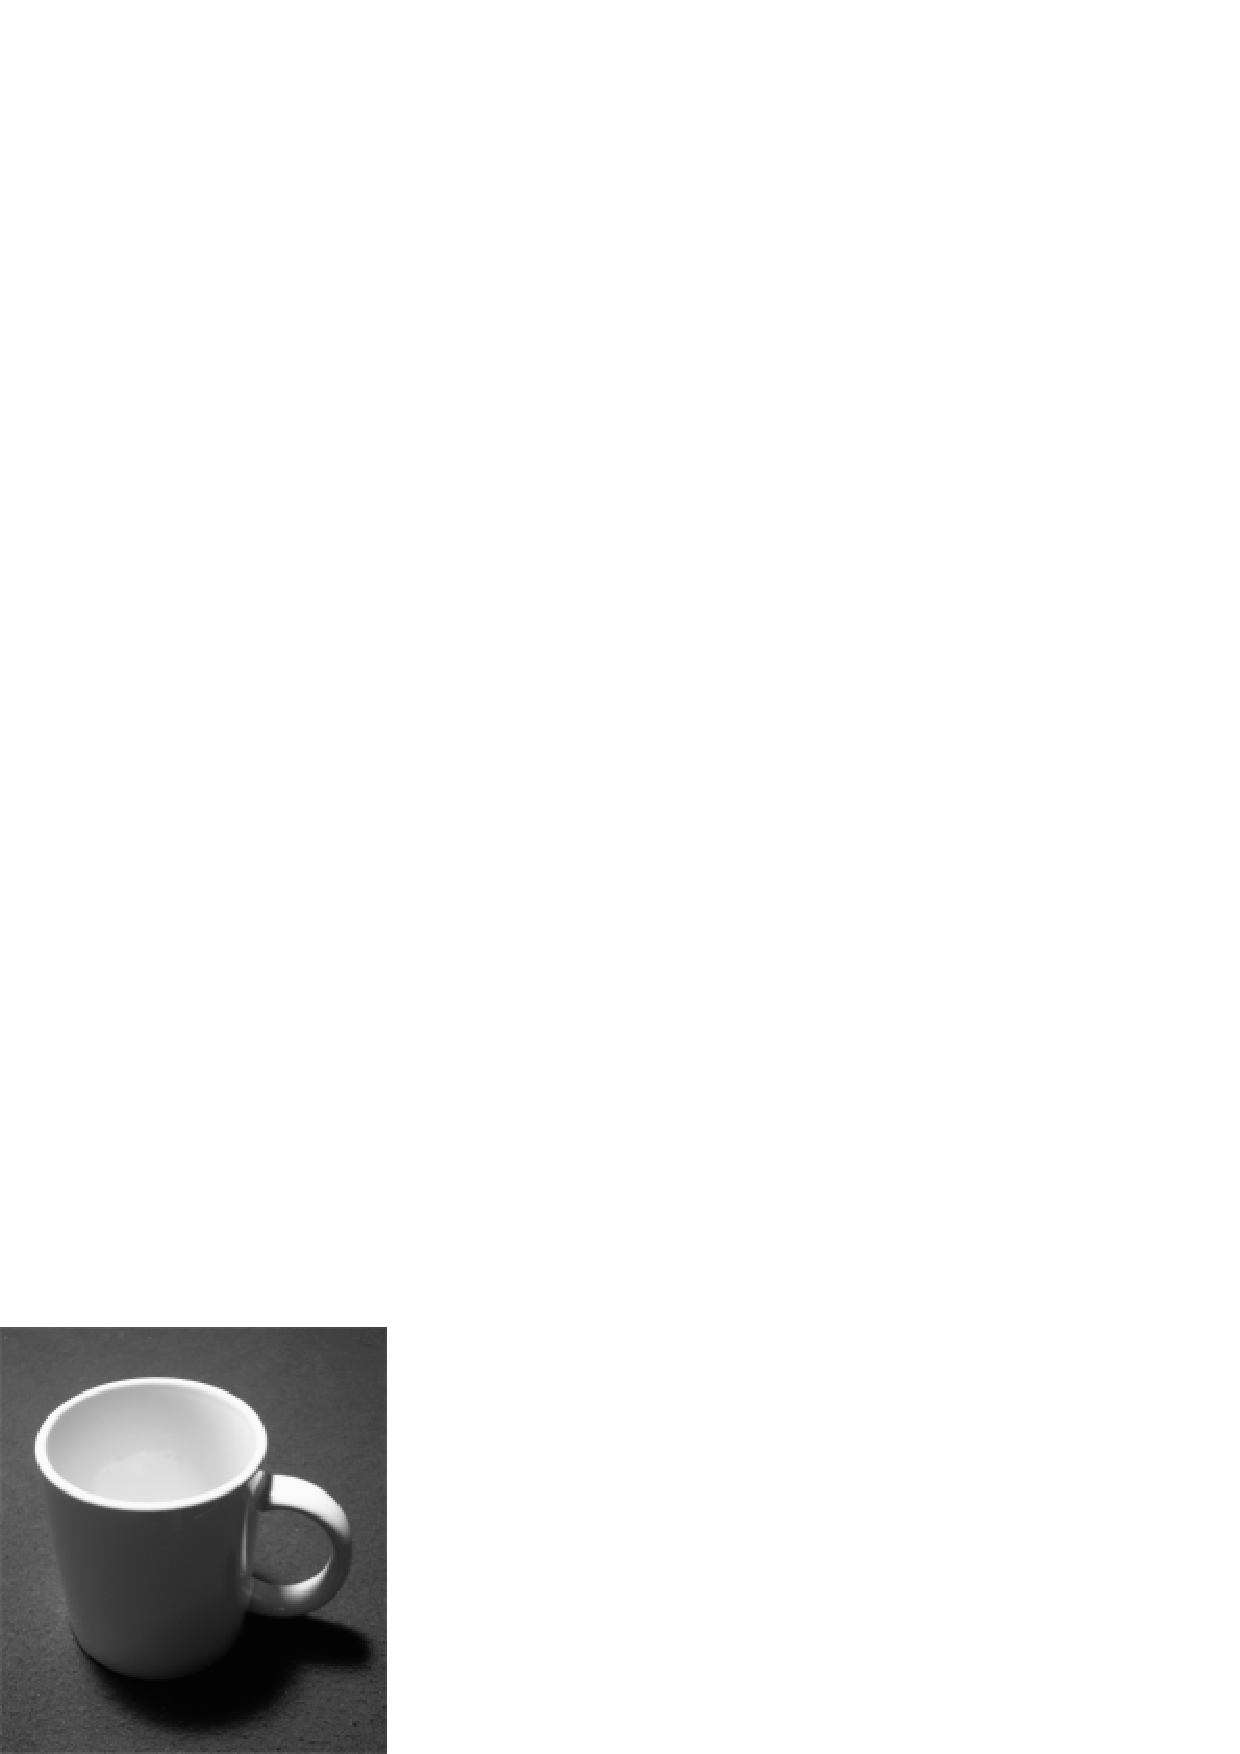
\includegraphics[height=0.08\textheight]{figs/grasping/mug.jpg} \\
      \includegraphics[height=0.08\textheight]{figs/grasping/grasp1.jpg}
      \includegraphics[height=0.08\textheight]{figs/grasping/grasp2.jpg}
      \includegraphics[height=0.08\textheight]{figs/grasping/grasp3.jpg}
      \includegraphics[height=0.08\textheight]{figs/grasping/grasp4.jpg}
      \includegraphics[height=0.08\textheight]{figs/grasping/grasp5.jpg} \\
    \end{tabular}
    \caption{(above) The devices and some of the objects used for the experiment,
    left to right: the CyberGlove, the Force Resistor Sensor attached
    to the subject's thumb, the beer can, the duct tape roll and the
    mug. (below) The $5$ grasp types to be recognized, left to right:
    power large, power flat, tripodal precision, thumb/index precision
    and spherical precision.}
    \label{fig:devices}
  \end{center}
\end{figure*}

%% The CyberGlove returns $22$ $8$-bit numbers linearly related to the
%% angles of the subject's hand joints; the sensors are embedded in the
%% glove in order for them to be adherent to the subject's skin. The
%% resolution of the sensors is on average about $0.5$ degree
%% \cite{cyberglove}, but the noise associated with the sensors has been
%% experimentally determined to be $1.1$ on average and $3$ at the
%% maximum \cite{212431}. The sensors describe the position of the three
%% phalanxes of each finger (for the thumb, rotation and two phalanxes),
%% the four finger-to-finger abductions, the palm arch, the wrist pitch
%% and the wrist yaw.

%% The FSR returns a $32$-bit number inversely related to the pressure
%% applied to the surface of the sensor. We used it as an on-off
%% indicator of when the subject was actually holding an
%% object. Toghether, the CyberGlove and FSR would give us a precise idea
%% of what the subject's hand posture was when grasping. All data were
%% collected, synchronised, and saved in real time at a frequency of
%% $50$Hz.

%% We then collected a number of objects encountered in everyday life,
%% and split them among $5$ pairs of sets, each set containing objects of
%% various size, colour, shape and affordances \cite{gibson}. The idea is
%% that each pair of sets would be associated with a particular type of
%% grasp, as identified by \cite{cutkosky}. The grasp types and
%% associated pairs were:

%% \begin{enumerate}
%%   \item \emph{power large grasp:} a beer can, a bottle and a box (set
%%     $1$); an anatomical hand model, a wooden toy dragon and a mug (set
%%     $2$);

%%   \item \emph{power flat grasp:} a hammer and a long Lego block (set
%%     $1$); a stapler, a screwdriver and and a TV remote control (set
%%     $2$);

%%   \item \emph{tripodal precision grip:} a small and a large ball, a
%%     rubber duck and a beer can (set $1$); a marker, a ballpoint pen
%%     and a ball (set $2$);

%%   \item \emph{thumb/index precision grip:} a knife, a duct tape roll,
%%     a short Lego block and a rubber duck (set $1$); a marker and a
%%     ballpoint pen (set $2$);

%%   \item \emph{spherical precision grip:} a small and a large ball and a
%%     rubber duck (set $1$); a fluffy toy airplane, a ball and a mug (set
%%     $2$).

%% \end{enumerate}

A number of objects encountered in everyday life were presented to the
subjects, who would then repeatedly grasp them in a particular way. The
grasp types were selected among those identified by Cutkosky in
\cite{cutkosky}: power large grasp, power flat grasp, tripodal
precision grip, thumb/index precision grip and spherical precision
grip. Figure \ref{fig:devices} shows three of the objects used in the
experiment and five examples of grasp types. Note that each object may
afford several grasp types, e.g., a rubber duck can be grasped either
via a tripodal precision grip, a thumb/index precision grip and/or a
spherical precision grip.

%% The experiment consisted of two phases. During the first phase, for
%% each pair, the first set of objects was put on the workspace, and the
%% subject was asked to choose one of the objects, grasp it with the
%% right hand, lift it and then put it back on the workspace. We
%% explicitly asked the subject to grasp \emph{using the grasp type
%% associated to the objects on the workspace}. We collected $60$ grasps
%% for each set of objects, resulting in $300$ grasps per subject,
%% divided by grasp type. During the second phase, we repeated the same
%% procedure but on a different day and using the second set of each
%% pair. Therefore, we would obtain analogous results to the first phase,
%% but allowing the subject to grasp different objects with the same
%% grasp type, and leaving a long time in between, in order for the
%% subject not to get used to a particular grasp type. Each phase was
%% completed by the subjects in $17$ to $18$ minutes.

%% In the end, this would allow us to gather $120$ grasps per grasp type
%% and subject; this means $960$ grasps per grasp type (for a total of
%% $4800$ grasps, since we had $5$ grasp types), well distributed across
%% various subjects, times of the day, fatigue conditions and objects.

%% The actual grasps, which would build the SVM training set, were
%% detected as follows: we found each interval of time during which the
%% FSR would signal contact, and then we took the CyberGlove sensors
%% values in the middle of the interval. We assumed that the hand posture would
%% not sensibly change during the grasping act, that is, while the subject
%% was lifting the object. Spurious grasp detections were removed from
%% the sample set, resulting in a total of $4512$ samples.

Each grasp is determined by the CyberGlove, therefore the input space
is $\RR^{22}$; and five categories, each corresponding to a grasp
type, were set up. The optimal hyperparameters $C$ and $\sigma$ were
found via grid search and cross-validation, as is customary.
%% The
%% machines were trained on data gathered during the first phase and
%% tested on data gathered during the second phase, and then
%% vice-versa. This way, the system was always tested on data related to
%% objects different from those seen during training, in order to remove
%% the possibility to learn the exact configuration of the hand rather
%% than the type of grasp.
We have compared OISVM with the batch method LIBSVM2 and the fixed-partition
technique. As in the experiments on place recognition experiments,
we have splitted the training data in several batches, to be able to use
the fixed partition method. In particular, in each training step we feed to
the systems all the data coming from an user.
A Gaussian kernel and three
different values of $\eta$ were used for OISVM. The results are shown
in Figure \ref{fig:exp:grasp}.

\begin{figure*}[t]
  \centering \footnotesize
  \begin{tabular}{c@{\hspace{0.5cm}}c}
    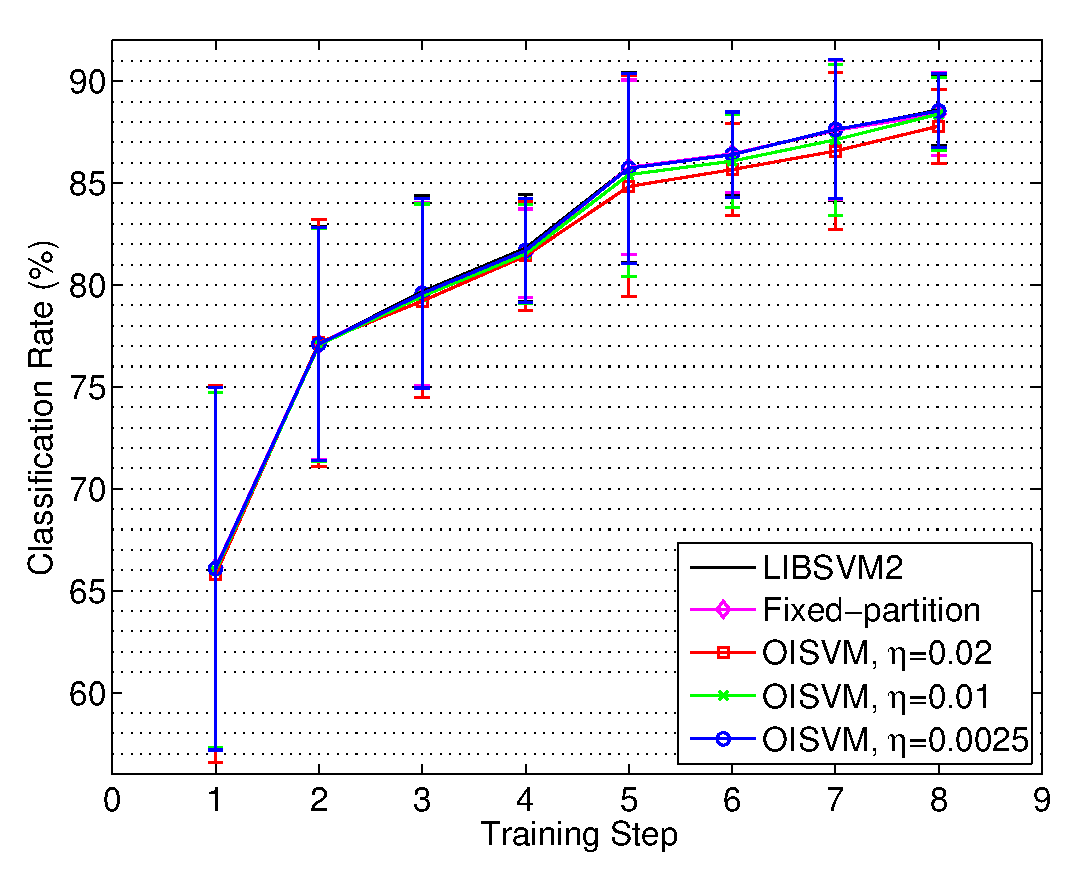
\includegraphics[width=0.47\linewidth]{figs/results/grasp_cr} &
    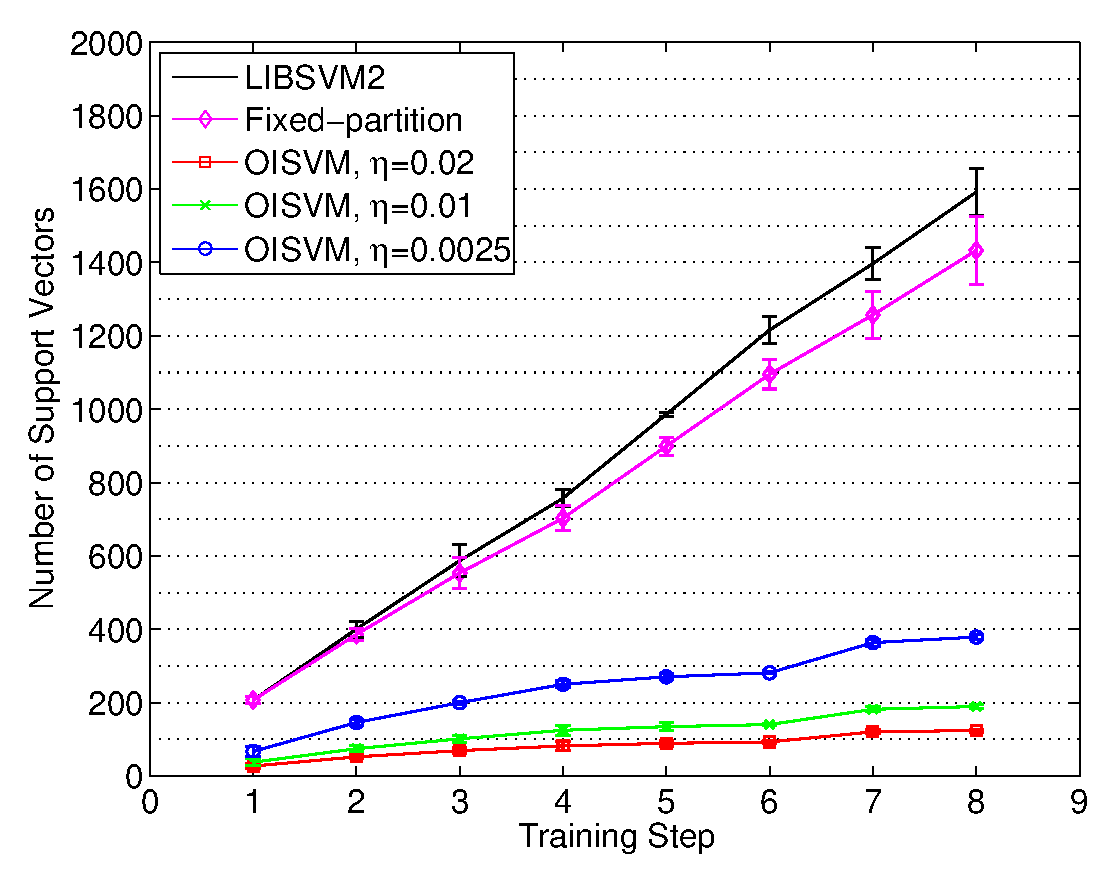
\includegraphics[width=0.47\linewidth]{figs/results/grasp_sv}
  \end{tabular}
  \caption{Classification rate (left) and average number of support
  vectors (left) for the grasping classification experiment. OISVM
  uses a Gaussian kernel and three different values of $\eta$.}
  \label{fig:exp:grasp}
\end{figure*}

Consider the Figure \ref{fig:exp:grasp}, left panel: it is apparent that the
classification rate is basically the same, uniformly and for all
approaches tested. The right panel shows that, in agreement with the
previous experiments, LIBSVM2 and the fixed partition method gather a
number of SVs which grows proportionally with the training set. On the
other hand, OISVM with various values of $\eta$ uniformly show a
dramatically smaller number of SVs, getting to as few as $124$ SVs in
the case for $\eta=0.02$, losing only $0.8\%$ of accuracy compared to
LIBSVM2.
